Das \textbf{DMX} (\textbf{D}ata \textbf{M}ultiple\textbf{x}ed) Protokoll
wurde erstmalig durch das USITT (United States Institute for Theatre
Technology) definiert. Es beschreibt die Steuerung von bis zu 512
Dimmern über eine serielle Verbindung. Das Protokoll findet
hauptsächlich in der Theater- und Bühenenbeleuchtungstechnik Anwendung.
Hierbei werden die Scheinwerfer über ein Busnetzwerk mit einem
Wertebereich von 8-bit gesteuert. Es gilt als State-of-the-art und ist
durch die DIN 56930-2 Norm definiert.\cite{dmx512/1990}

\hypertarget{funktionsweise-des-protokolls}{%
\subsection{Funktionsweise des
Protokolls}\label{funktionsweise-des-protokolls}}

Die Informationen werden im DMX Protokoll digital übertragen, wobei hier
zwischen einer positiven und negativen Spannung von ungefähr 2,5 Volt
unterschieden wird. Ein Einser entspricht einer positiven Spannung für 4
\textmu s und ein Nuller einer negativen Spannung für die selbe
Zeitspanne. DMX verwendet eine 8-bit Datenlänge. Der Wertebereich eines
Kanals liegt also zwischen Null und 255. Die jeweiligen Werte für jeden
Kanal werden nacheinander gesendet. Am Anfang jedes Signals wird eine
Reset-Sequenz gefolgt von einem Startbyte gesendet.\cite{dmx-1} Siehe
Bild \ref{dmx-signal}.

\begin{figure}
\centering
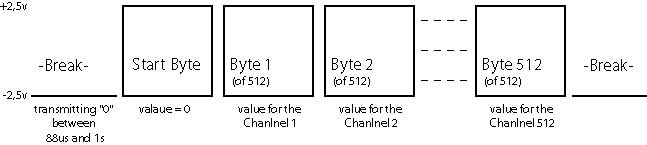
\includegraphics{bilder/Clemens/dmx.jpg}
\caption{Darstellung des DMX-Signals\label{dmx-signal}}
\end{figure}

Der Vorteil dieses Protokolls ist, dass alle Empfänger nur an ein Kabel
angeschlossen werden müssen und die meist schon vorhandene
XLR-Verkabelung genutzt werden kann.\cite{dmx512/1990}

Ein Nachteil ist, dass bei vielen genutzten Kanälen das Signal und somit
auch die Refreshrate sehr gering wird. Das bedeutet, dass in der Praxis
DMX mit weniger Geräten betrieben werden sollte.\cite{dmx512/1990}

\hypertarget{anwendung-in-diesem-projekt}{%
\subsection{Anwendung in diesem
Projekt}\label{anwendung-in-diesem-projekt}}

In diesem Projekt wurde DMX als Schnittstelle zur Beleuchtung
integriert. Dadurch bleibt das System flexibel, so gibt der
Administrator bei der Installation nur an welcher Kanal, welchem
Scheinwerfer zuzuordnen ist. Weiters wird dadurch auch garantiert, dass
das System mit allen DMX-Stanadard konformen Scheinwerfern funktioniert.
Ein weiterer Vorteil, der sich durch die Integration des Protokolls
ergibt, ist, dass nicht nur Dimmer, sondern auch RGB- und
RGBW-Scheinwerfer gesteuert werden können. Die Art des Scheinwerfers
wird an der Anzahl der durch den Administrator angegebenen Kanäle pro
Scheinwerfer bestimmt. So ist es auch möglich, dass verschiedene Typen
gemischt werden können.

Wenn vom User der Befehl zur Änderung einer Einstellung an einem der
Scheinwerfer gesendet wird, wird im Hintergrund das zu diesem
Scheinwerfer passende Scheinwerfer-Objekt aufgerufen, welches über die
Php-Extension (siehe \ref{PHP-Extension}) und Ola (siehe \ref{Ola}) den
entsprechenden Wert des DMX-Kanals ändert.
